%---------------------------
% CHAPTER 7: Implementation
%---------------------------

\chapter{Implementation}

\label{chapter07}

Once the system is designed and its architecture defined, the implementation took an important part of the time. The \thesis\ used a lot of frameworks and libraries that eased the development. Some of them has been already explained, like \nameref{apache_spark} that offers an API to process big data dumps and it parallelizes the process automatically.
\\\\
First of all, lets check the main programming languages used in this project and then all libraries and frameworks component by component, finally the tools used for the development.

\section{Programming languages}

\subsection*{Scala\cite{scala}}

\begin{figure}[H]

\includegraphics[scale=0.1]{resources/scala-logo.png}
\end{figure}

Scala (\texttt{.scala} as file extension) is multi-paradigm programming language compiled by the Java Virtual Machine\cite{jvm}. Its main paradigms are \textbf{functional}, very useful for \nameref{apache_spark}, Java\cite{java} also provides this since version 8, but in Scala it is much easier to write and debug; Scala is also object-oriented, imperative and concurrent.
\\\\
Scala is the preferred language by the Apache Software Foundation for \nameref{apache_spark}, that is why it is the main language used in both pipelines, \nameref{available-flights-pipeline} and \nameref{user-searches-pipeline}. The latest \nameref{apache_spark} is for Scala, then it usually comes out for Java and finally for Python.
\\\\
I have never programmed in Scala before this project, but it was very fast and easy to learn. Knowing Java, the syntax is not much different and, usually, more intuitive.

\subsection*{Python\cite{python}}

\begin{figure}[H]

\includegraphics[scale=0.1]{resources/python-logo.png}
\end{figure}

Python (with file extension \texttt{.py}) is the language used for the service. Python 3.6 is the version used instead of 2.7, which is very different, because Python2.7 will not have support anymore in a few months.
\\\\
The syntax of python is different than C based languages and allows a lot of \textit{tricks} that the developer cannot do in most programming languages, for instance: \texttt{array[-1]} gets the last element. It is the only language used in the \nameref{comparison_service}, thanks to Python's flexibility; imperative, functional, object-oriented, procedure and reflective paradigms; duck, string and dynamic typing and compatibility with lost of technologies makes the service easy to be implemented in few lines.

\subsection*{JavaScript\cite{js}}

Often abbreviated as JS, JavaScript is an interpreted programming language core of the World Wide Web technologies all along with HTML\cite{html} and CSS\cite{css}. It is used in the \nameref{web-ui} and, like Python, it has compatibility with a lot of technologies, \nameref{axios}, \nameref{reactjs} and \nameref{vega} for this project.

\begin{figure}[H]

\includegraphics[scale=0.1]{resources/www-tech-logos.jpeg}
\caption{HTML 5, JavaScript and CSS 3 logos.}
\end{figure}

\section{External libraries and frameworks}

\subsection*{Scala Amazon Web Service's Software Development Kit\cite{scala_aws}} \label{scala_aws}

Amazon provides a lot of APIs for different programming languages. The AWS SDK for Java enable Java developers to easily work with Amazon Web Services and build scalable solutions with Amazon S3, Amazon Athena, Amazon DynamoDB, and more. Since Scala is assembled by the Java Virtual Machine, Amazon created the Scala Amazon Web Services SDK, it's like the AWS SDK for Java, but more Scala-y.
\\\\
Thanks to that Software Development Kit both pipelines can write to the \nameref{s3} and query \nameref{athena} in the case of the User Searches Pipeline.

\subsection*{Boto3\cite{boto3}} \label{boto3}

This Python library is also very important for the project. It is the Amazon Web Service's Software Development Kit for Python. It is not as complete as the Java AWS SDK or the Scala AWS SDK but the \nameref{s3} API is more than enough for the Comparison Service.

\subsection*{aiohttp\cite{aiohttp}} \label{aiohttp}

In order to have an Asynchronous HTTP Client and Service for Python, the \thesis\ is using AIOHTTP. One of its key features is the support to Server WebSockets.

\subsection*{axios\cite{axios}} \label{axios}

For the \nameref{web-ui} to call the \nameref{comparison_service}, axios is a JavaScript library that provides a promise based HTTP client for the browser.

\subsection*{React.js\cite{reactjs}} \label{reactjs}

React is a set of libraries combined in a single framework for building user interfaces in JavaScript. Allows the developer create a Declarative and Component-Based interface. React is build a way that when a change happens it does not render all the page again, it only renders the component that has changed, making the website much faster than typical static pages.

\subsection*{Vega\cite{vega}} \label{vega}

Interactive Data Lab created Vega and Vega Lite, a library that allows create visualization designs using a declarative format. All visualizations are described in JSON\cite{json} and Vega does all the work for you. The \nameref{web-ui} uses the Line Chart provided by Vega Lite.

\begin{figure}[H]
\centering
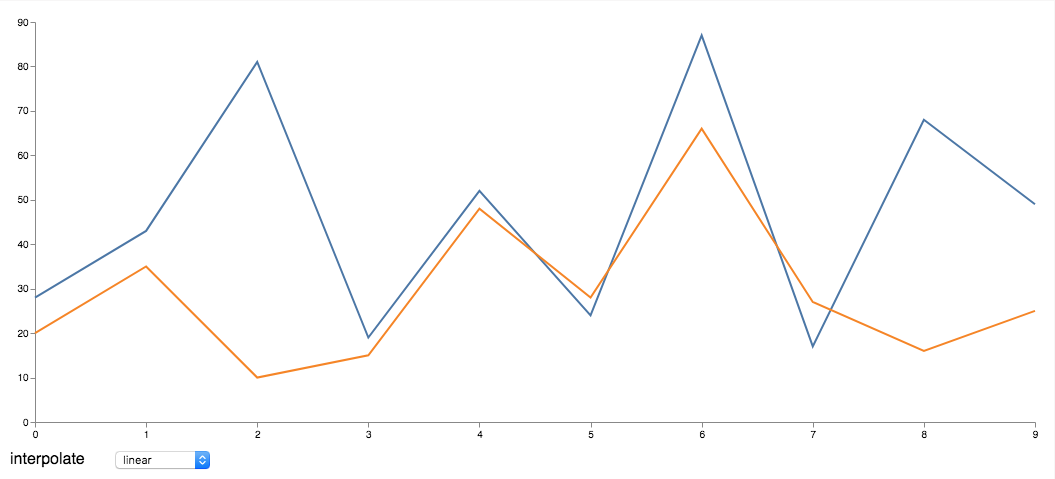
\includegraphics[scale=0.4]{resources/lineal-chart-example01.png}
\caption{Vega Lite line chart example.}
\end{figure}

\section{Developing tools}

The two main tools used for the development of the \thesis\ are IntelliJ IDEA by JetBrains and Sublime Text 3.

\subsection*{IntelliJ IDEA by JetBrains\cite{intellij}}

\begin{figure}[H]

\includegraphics[scale=0.1]{resources/intellij-logo.png}
\end{figure}

\textit{Capable and Ergonomic IDE for JVM}. IntelliJ is the preferred IDE\cite{ide} in \company. Ease the development of Java projects and, with a Scala Building Tool plugin IntelliJ eases the development of Scala projects. This Integrated Development Environment has been used for writing, testing, executing and assembling \nameref{available-flights-pipeline} and \nameref{user-searches-pipeline}.

\subsection*{Sublime Text 3\cite{sublimetext}}

\begin{figure}[H]

\includegraphics[scale=0.1]{resources/sublime-logo.png}
\end{figure}

Sublime Text is not an IDE, is just a text editor for code, markup and prose. Sophisticated and full of features for the developers, makes easier the development of software, systems and applications that do not have an specific IDE or that the existing development environment complicates the project. That is why Sublime Text 3 has been used for the \nameref{comparison_service} and the \nameref{web-ui}.



